% -*- coding: utf-8 -*-

\documentclass[10pt,dvipdfmx]{beamer}
\usepackage{tutorial}

\title{計算機実験I (講義4)}
\date{2022/06/29}

\begin{document}

\begin{frame}
  \titlepage
  \tableofcontents
  出席: 本日の18時までにITC-LMSでアンケートに回答
\end{frame}

\section{行列の対角化}
% -*- coding: utf-8 -*-

\documentclass[10pt,dvipdfmx]{beamer}
\usepackage{tutorial}

\begin{document}
\section{行列とLAPACK}
\begin{frame}[t,fragile]{二次元配列}
  \begin{itemize}
    %\setlength{\itemsep}{1em}
  \item C言語では、二次元配列は一次元配列の先頭をさす(ポインタ)の配列として表される(と理解しておけば良い)
  \item \verb+a[i]+は、要素\verb+a[i][0]+を指すポインタ
    \begin{itemize}
    \item \verb+a+ と \verb+&a[0]+ は等価 (\verb+&a[0][0]+ ではない)
    \item \verb+a[0]+ と \verb+&a[0][0]+ は等価
    \item \verb+a[2]+ と \verb+&a[2][0]+ は等価
    \item \verb^(a+2)^ と \verb^&a[2]^ は等価
    \item \verb^(*(a+2))[3]^ と \verb^*(*(a+2)+3)^ と \verb^a[2][3]^ は等価
    \item \verb^*(a+2)[3]^ と \verb^*((a+2)[3])^ と \verb^*(a[5])^ と\verb^a[5][0]^ は等価
    \item \verb^[]^は\verb^*^よりも優先度が高い
    \end{itemize}
  \item ポインタのテストプログラム: \href{https://github.com/todo-group/computer-experiments/blob/master/exercise/matrix/pointer-matrix.c}{pointer-matrix.c}
  \end{itemize}
\end{frame}

\begin{frame}[t,fragile]{動的二次元配列の確保}
  \begin{itemize}
    \setlength{\itemsep}{1em}
  \item 各行を表す配列とそれぞれの先頭アドレスを保持する配列の二種類が必要
\begin{lstlisting}
double **a;
m = 10;  
n = 10;  
a = (double**)malloc((size_t)(m * sizeof(double*));
for (int i = 0; i < m; ++i)
  a[i] = (double*)malloc((size_t)(n * sizeof(double));
\end{lstlisting}
\item 各行を保持する配列が、メモリ上で連続に確保される保証はない
\item 行列用のライブラリ(LAPACK等)を使うときに問題となる
  \end{itemize}
\end{frame}

\begin{frame}[t,fragile]{BLASライブラリ}
  \begin{itemize}
    \setlength{\itemsep}{1em}
  \item 行列・行列積、行列・ベクトル積などを高速に行う最適化された関数群
  \item 行列・行列積を計算するサブルーチン {\tt dgemm} \\
    \url{http://www.netlib.org/lapack/explore-html/d7/d2b/dgemm_8f.html}
    \begin{itemize}
    \item $C = \alpha A \times B + \beta C$ を計算
    \item BLASもFortranで書かれている
    \end{itemize}
  \item 例: \href{https://github.com/todo-group/computer-experiments/blob/master/exercise/matrix/multiply.c}{multiply.c}, \href{https://github.com/todo-group/computer-experiments/blob/master/exercise/matrix/multiply_dgemm.c}{multiply\_dgemm.c}
  \end{itemize}
\end{frame}

\begin{frame}[t,fragile]{LAPACK (Linear Algebra PACKage)}
  \begin{itemize}
    %\setlength{\itemsep}{1em}
  \item 線形計算のための高品質な数値計算ライブラリ
    \begin{itemize}
    \item \url{http://www.netlib.org/lapack}
    \item 線形方程式、固有値問題、特異値問題、線形最小二乗問題など
    \item (FFT 高速フーリエ変換は入っていない)
    % \item LAPACK自体もFortran言語で書かれている
    \end{itemize}
  \item ほぼ全てのPC、ワークステーション、スーパーコンピュータで利用可 (インストール済)
  \item Netlibでソースが公開されているリファレンス実装は遅いが、それぞれのベンダー(Intel、Fujitsu、etc)による最適化されたLAPACKが用意されている場合が多い(MKL、SSL2、etc)
  \item LAPACKを使うことにより、高速で信頼性が高く、ポータブルなコードを書くことが可能になる
  \end{itemize}
\end{frame}

\begin{frame}[t,fragile]{LAPACKによる連立一次方程式の求解}
  \begin{itemize}
    \setlength{\itemsep}{1em}
  \item LU分解を行うサブルーチン {\tt dgetrf} \\
    \url{http://www.netlib.org/lapack/explore-html/d3/d6a/dgetrf_8f.html}
  \item Fortranによる関数宣言
\begin{lstlisting}
subroutine dgetrf(integer M, integer N,
         double precision, dimension(lda, *) A,
         integer LDA, integer, dimension(*) IPIV,
         integer INFO)
\end{lstlisting}
\item {\tt A}: 左辺の行列、{\tt M,N}: 次元、{\tt IPIV}: 選択されたピボット行のリスト、{\tt lda}: 通常{\tt M} (行数)と同じで良い
  \end{itemize}
\end{frame}

\begin{frame}[t,fragile]{CからBLAS/LAPACKを呼び出す際の注意事項}
  \begin{itemize}
    %\setlength{\itemsep}{1em}
  \item (もともとFortran言語で書かれていたことによる制限)
  \item 関数名はすべて小文字、最後に \verb+_+ (下線)を付ける
  \item スカラー、ベクトル、行列は全て「ポインタ渡し」とする
  \item ベクトルや行列は最初の要素へのポインタを渡す (サイズは別に渡す)
  \item 行列の要素は(0,0) $\rightarrow$ (1,0) $\rightarrow$ (2,0) $\rightarrow\cdots\rightarrow$ $(m-1,0)$ $\rightarrow$ (0,1) $\rightarrow$ (1,1) $\rightarrow\cdots\rightarrow$ $(m-1,n-1)$の順で連続して並んでいなければならない(column-major)
    \begin{itemize}
    \item C言語の二次元配列では \verb+a[i][j]+ の次には \verb%a[i][j+1]%が入っている(row-major)
    \item 行列が転置されて解釈されてしまう!
    \end{itemize}
  \item コンパイル時には{\tt -llapack -lblas}オプションを指定し、LAPACKライブラリとBLASライブラリをリンクする(ハンドブック2.1.6節)
  \end{itemize}
\end{frame}

\begin{frame}[t,fragile]{cmatrix.hライブラリ}
  \begin{itemize}
    %\setlength{\itemsep}{1em}
  \item Column-major形式の二次元配列の確保({\tt alloc\_dmatrix})、開放({\tt free\_dmatrix})、出力({\tt print\_dmatrix})、読み込み({\tt read\_dmatrix})を行うためのユーティリティ関数、(i,j)成分にアクセスするためのマクロ({\tt mat\_elem})他を準備
  \item ソースコード: \href{https://github.com/todo-group/computer-experiments/blob/master/exercise/matrix/cmatrix.h}{cmatrix.h}
  \item 使用例
\begin{lstlisting}
#include "cmatrix.h"
...
double **mat;
mat = alloc_dmatrix(m, n);
mat_elem(mat, 1, 3) = 5.0;
...
free_dmatrix(mat);
\end{lstlisting}
  \item サンプルコード: \href{https://github.com/todo-group/computer-experiments/blob/master/exercise/matrix/matrix_example.c}{matrix\_example.c}
  \end{itemize}
\end{frame}

\begin{frame}[t,fragile]{alloc\_dmatrixでの動的二次元配列の確保}
  \begin{itemize}
    %\setlength{\itemsep}{1em}
  \item 長さ$m \times n$の一次元配列を用意し、各列(それぞれ$m$要素)の先頭アドレスを長さ$n$のポインター配列に格納する (ハンドブック2.12.3節)
\begin{lstlisting}
double **a;
m = 10;  
n = 10;  
a = (double**)malloc((size_t)(n * sizeof(double*));
a[0] = (double*)malloc((size_t)(m*n * sizeof(double));
for (int i = 1; i < n; ++i)
  a[i] = a[i-1] + m;
\end{lstlisting}
\item 行列の(i,j)成分を\verb+a[j][i]+に格納することにする (column-major)
  \end{itemize}
\end{frame}

\begin{frame}[t,fragile]{要素アクセス・先頭アドレス}
  \begin{itemize}
    % \setlength{\itemsep}{1em}
  \item 行列の(i,j)成分は\verb+a[j][i]+に格納されている
    \begin{itemize}
      \item \href{https://github.com/todo-group/computer-experiments/blob/master/exercise/matrix/cmatrix.h}{cmatrix.h}ではマクロ(\verb+mat_elem+)を準備
\begin{lstlisting}
#define mat_elem(mat, i, j) (mat)[j][i]
\end{lstlisting}
\item このマクロを使うと、例えば(i,j)成分への代入は以下のように書ける
\begin{lstlisting}
mat_elem(a, i, j) = 1;
\end{lstlisting}
\end{itemize}
  \item LAPACKにベクトルや行列の最初の要素へのポインタを渡す
    \begin{itemize}
      \item ベクトルの最初の要素(0)へのポインタ: \verb+&v[0]+
      \item 行列の最初の要素(0,0)へのポインタ: \verb+&a[0][0]+
      \item \href{https://github.com/todo-group/computer-experiments/blob/master/exercise/matrix/cmatrix.h}{cmatrix.h}にマクロ({\tt vec\_ptr}、{\tt mat\_ptr})が準備されているのでそれぞれ、{\tt vec\_ptr(v)}、{\tt mat\_ptr(a)}と書ける
    \end{itemize}
  \end{itemize}
\end{frame}

\begin{frame}[t,fragile]{LAPACKによる連立一次方程式の求解}
  \begin{itemize}
    \setlength{\itemsep}{1em}
  \item C言語から呼び出すための関数宣言を作成 (ハンドブック2.7.4節)
\begin{lstlisting}
void dgetrf_(int *M, int *N, double *A,
             int *LDA, int*IPIV, int *INFO);
\end{lstlisting}
関数名は全て小文字。関数名の最後に {\tt \_} (下線)を付ける
\item LU分解の例
\begin{lstlisting}
m = 10;
n = 10;
a = alloc_dmatrix(m, n);
...
dgetrf_(&m, &n, mat_ptr(a), &m, vec_ptr(ipiv), &info);
\end{lstlisting}
完全なソースコード: \href{https://github.com/todo-group/computer-experiments/blob/master/exercise/linear_system/lu_decomp.c}{lu\_decomp.c}
  \end{itemize}
\end{frame}

\end{document}

\begin{frame}[t,fragile]{時間依存しないシュレディンガー方程式}
  \begin{itemize}
    \setlength{\itemsep}{1em}
  \item 井戸型ポテンシャル中の一粒子問題
    \begin{align*}
      \big[ -\frac{\hbar^2}{2m}\frac{d^2}{dx^2} + V(x) \big] \psi(x) = E \psi(x) \\
      V(x) = \begin{cases}
        0 & \text{$a \le x \le b$} \\ \infty & \text{otherwise}
      \end{cases}
    \end{align*}
  \item $\hbar^2/2m = 1$、$a=0$、$b=1$となるように変数変換して
    \begin{align*}
      \big( \frac{d^2}{dx^2} + E \big) \psi(x) = 0 \qquad 0 \le x \le 1
    \end{align*}
    を境界条件$\psi(0) = \psi(1) = 0$のもとで解けば良い
  \end{itemize}
\end{frame}

%\begin{frame}[t,fragile]{ポアソン方程式の境界値問題}
  \begin{itemize}
    %\setlength{\itemsep}{1em}
  \item 二次元ポアソン方程式
    \[ \frac{\partial^2 u(x,y)}{\partial x^2} + \frac{\partial^2 u(x,y)}{\partial y^2} = f(x,y) \qquad 0 \le x \le 1, \ 0 \le y \le 1\]
  \item ディリクレ型境界条件: $u(x,y) = g(x,y)$ on $\partial \Omega$
  \item 有限差分法により離散化
    \begin{itemize}
    \item $x$方向、$y$方向をそれぞれ$n$等分: $(x_i,y_j) = (i/n, j/n)$
    \item $(n+1)^2$個の格子点の上で$u(x_i,y_j)=u_{ij}$が定義される
    \item そのうち$4n$個の値は境界条件で定まる
    \item ポアソン方程式を中心差分で近似 ($h=1/n$)
      \[
      \frac{u_{i+1,j}-2u_{ij}+u_{i-1,j}}{h^2} + \frac{u_{i,j+1}-2u_{ij}+u_{i,j-1}}{h^2} = f_{ij}
      \]
      残り$(n-1)^2$個の未知数に対する連立一次方程式
    \end{itemize}
  \end{itemize}
\end{frame}

\begin{frame}[t,fragile]{シュレディンガー方程式の行列表示}
  \begin{itemize}
    %\setlength{\itemsep}{1em}
  \item シュレディンガー方程式
    \[
    [-\frac{d^2}{dx^2}+V(x)]\psi(x) = E \psi(x)
    \]
  \item 連立差分方程式を行列の形で表す($\psi(x_0)=\psi(x_n)=0$)
    \begin{footnotesize}
    \[
    \begin{pmatrix}
      \frac{2}{h^2}+V(x_1) & -\frac{1}{h^2} \\
      -\frac{1}{h^2} & \frac{2}{h^2}+V(x_2) & -\frac{1}{h^2} \\
      & -\frac{1}{h^2} & \frac{2}{h^2}+V(x_3) & -\frac{1}{h^2} \\
      & & \ddots & \ddots \\
      & & & -\frac{1}{h^2} & \frac{2}{h^2}+V(x_{n-1}) \\
    \end{pmatrix}
    \begin{pmatrix}
      \psi(x_1) \\
      \psi(x_2) \\
      \psi(x_3) \\
      \vdots \\
      \psi(x_{n-1}) \\
    \end{pmatrix}
    = \cdots % E
    %% \begin{pmatrix}
    %%   \psi(x_1) \\
    %%   \psi(x_2) \\
    %%   \psi(x_3) \\
    %%   \vdots \\
    %%   \psi(x_{n-1}) \\
    %% \end{pmatrix}
    \]
    \end{footnotesize}
  \item $(n-1) \times (n-1)$の疎行列の固有値問題
    \begin{itemize}
    \item 固有値: 固有エネルギー
    \item 固有ベクトル: 波動関数
    \end{itemize}
  \end{itemize}
\end{frame}

\begin{frame}[t,fragile]{固体物理・量子統計物理に現れる行列}
  \begin{itemize}
    %\setlength{\itemsep}{1em}
  \item 強束縛近似(tight-binding approx.)のもとでの第二量子化表示
    \[
    H = -t \sum_{\langle i,j \rangle \sigma} (c_{i,\sigma}^\dagger c_{j,\sigma} + h.c.) + \text{(相互作用)}
    \]
  \item 局所スピン模型(ハイゼンベルグ模型)
    \[
    H = -J\sum_{\langle i,j \rangle} S_i \cdot S_j
    = -J\sum_{\langle i,j \rangle} [S_i^z S_j^z +\frac{1}{2} (S_i^+ S_j^- + S_i^- S_j^+) ]
    \]
  \item 格子点の数を$n$とすると、ハミルトニアンはそれぞれ$4^n \times 4^n$、$2^n \times 2^n$の(疎)行列で表される。
  \item $n$が大きくなると、行列の次元は指数関数的に増加
  \item 量子多体系に共通する困難
  \end{itemize}
\end{frame}

\begin{frame}[t,fragile]{実対称行列(エルミート行列)の性質}
  \begin{itemize}
    %\setlength{\itemsep}{1em}
  \item $N \times N$実対称行列$A$ ($=A^T$)の固有値問題
    \[
    A x = \lambda x
    \]
  \item $N$個の固有値($\lambda_1,\lambda_2,\cdots,\lambda_N$)は全て実。固有ベクトル($\xi_1,\xi_2,\cdots,\xi_N$)は互いに正規直交するようにとることができる。行列$U$を
    \[
    U = \Big( \xi_1 \, \xi_2 \, \cdots \, \xi_N \Big)
    \]
    と定義すると、$U$は直交(ユニタリ)行列($U^T U = U^{-1} U = I$)
  \item $A$の固有分解(固有値分解)
    \[
    A = U \Lambda U^T \qquad \Lambda = \text{diag}(\lambda_1,\cdots,\lambda_N)
    \]
  \end{itemize}
\end{frame}

\begin{frame}[t,fragile]{行列のべき乗・指数関数}
  \begin{itemize}
    %\setlength{\itemsep}{1em}
  \item 行列のべき乗
    \begin{align*}
      A^p &= (U \Lambda U^T)(U \Lambda U^T) \cdots (U \Lambda U^T) \\
      &= U \Lambda^p U^T \qquad \Lambda^p = \text{diag}(\lambda_1^p,\cdots,\lambda_N^p)
    \end{align*}
  \item 行列の指数関数
    \begin{align*}
      e^{xA} &= \sum_{n=0}^{\infty} \frac{1}{n!}(xA)^n = U \Big[ \sum_{n=0}^{\infty} \frac{1}{n!}(x\Lambda)^n \Big] U^T \\
      &= U e^{x \Lambda} U^T \qquad e^{x \Lambda} = \text{diag}(e^{x\lambda_1},\cdots,e^{x\lambda_N})
    \end{align*}
  \item 逆行列 $A^{-1} = U \Lambda^{-1} U^T$
  \item 行列式 $|A| = \prod_i \lambda_i$、対角和(トレース) ${\rm tr} A = \sum_i \lambda_i$
  \end{itemize}
\end{frame}

\begin{frame}[t,fragile]{行列の数値対角化}
  \begin{itemize}
    %\setlength{\itemsep}{1em}
  \item 一般的に次元が5以上の行列の固有値は、あらかじめ定まる有限回の手続きでは求まらない
    \begin{itemize}
    \item 必ず何らかの反復法(+収束判定)が必要となる
    \end{itemize}
  \item 密行列向きの方法
    \begin{itemize}
    \item Jacobi法
    \item Givens変換・Householder法(三重対角化) + QR法など
    \end{itemize}
  \item 疎行列向きの方法
    \begin{itemize}
    \item べき乗法
    \item Lanczos法(三重対角化) + QR法など
    \end{itemize}
  \item 固有ベクトル
    \begin{itemize}
    \item QR法で求めたものを逆変換
    \item 逆反復法で精度改善
    \end{itemize}
  \end{itemize}
\end{frame}


\section{密行列の対角化}

\begin{frame}[t,fragile]{基本方針}
  \begin{itemize}
    %\setlength{\itemsep}{1em}
  \item やってはいけない方法: 特性方程式
    \[
    |\lambda E - A| = 0
    \]
    の係数を求めて、代数方程式として解く
    \begin{itemize}
    \item 数値的に不安定 (代数方程式の解は係数の誤差に対して敏感)
    \item 計算コスト大[$\sim O(N!)$]
    \end{itemize}
  \item スタンダードな方法: 行列を次々に直交変換して、対角行列(あるいは三重対角行列)に近づけていく
    \[
    A \rightarrow U_1^T A U_1 \rightarrow U_2^T (U_1^T A U_1) U_2 \rightarrow U_3^T (U_2^T (U_1^T A U_1) U_2) U_3 \rightarrow \cdots
    \]
  \item 固有値は変換された行列の固有値、固有ベクトルは変換後の行列の固有ベクトルに左から$U_1 U_2 U_3 \cdots$を掛けたもの
  \end{itemize}
\end{frame}

\begin{frame}[t,fragile]{Jacobi法}
  \begin{itemize}
    \setlength{\itemsep}{1em}
  \item 直交行列$U_{pq}$を以下のように選ぶ ($(p,p),(p,q),(q,p),(q,q)$成分を除くと単位行列)
    \[
    U_{pq} =
    \begin{bmatrix}
      1 \\
      & \ddots \\
      & & 1 \\
      & & & \cos \theta & & & \sin \theta \\
      & & & & 1 \\
      & & & & & 1 \\
      & & & -\sin \theta & & & \cos \theta \\
      & & & & & & & 1 \\
      & & & & & & & & \ddots \\
      & & & & & & & & & 1 \\
    \end{bmatrix}
    \]
  \end{itemize}
\end{frame}

\begin{frame}[t,fragile]{Jacobi法による相似変換}
  \begin{itemize}
    %\setlength{\itemsep}{1em}
  \item $B=U_{pq}^{-1} A U_{pq}$により、$A$の$p$行、$q$行、$p$列、$q$列のみが変更を受ける
    \begin{align*}
      b_{pk} &= b_{kp} = a_{pk} \cos \theta - a_{qk} \sin \theta \qquad k \ne p,q \\
      b_{qk} &= b_{kq} = a_{pk} \sin \theta + a_{qk} \cos \theta \qquad k \ne p,q \\
      b_{pp} &= \frac{a_{pp}+a_{qq}}{2} + \frac{a_{pp}-a_{qq}}{2} \cos 2 \theta - a_{pq} \sin 2 \theta \\
      b_{qq} &= \frac{a_{pp}+a_{qq}}{2} - \frac{a_{pp}-a_{qq}}{2} \cos 2 \theta + a_{pq} \sin 2 \theta \\
      b_{pq} &= b_{qp} = \frac{a_{pp}-a_{qq}}{2} \sin 2 \theta + a_{pq} \cos 2 \theta
    \end{align*}
  \item $b_{pq} = b_{qp} = 0$とするには、$\theta$を次のように選べば良い
    \[
    \tan 2 \theta = - \frac{2 a_{pq}}{a_{pp}-a_{qq}}
    \]
  \end{itemize}
\end{frame}

\begin{frame}[t,fragile]{Jacobi法の収束}
  \begin{itemize}
    %\setlength{\itemsep}{1em}
  \item 相似変換により対角和は不変に保たれるので
    \[
      {\rm tr} \, A^T A = {\rm tr} \, B^T B \ \ \Rightarrow \ \
      \sum_{i,j} a_{ij}^2 = \sum_{i,j} b_{ij}^2
    \]
  \item 一方、この変換で
    \[
    b_{pp}^2 + b_{qq}^2 = b_{pp}^2 + 2 b_{pq}^2 + b_{qq}^2 = a_{pp}^2 + 2 a_{pq}^2 + a_{qq}^2
    \]
    すなわち、変換により、対角成分の二乗和は増加する $\Rightarrow$ 非対角成分の二乗和は単調減少
  \item 全ての非対角成分が十分小さくなるまで繰り返す
  \item 固有値=対角成分、固有ベクトル$=U_1 U_2 U_3 \cdots$
  \end{itemize}
\end{frame}

\begin{frame}[t,fragile]{3重対角化}
  \begin{itemize}
    %\setlength{\itemsep}{1em}
  \item 対角化は有限回の手続きでは行えない
  \item 3重対角化であれば、$O(n^3)$の有限回の計算で決定論的に行える
  \item Givens変換: Jacobi変換と同じ相似変換を利用
    \begin{itemize}
    \item $U_{32}$で(3,1)と(1,3)を消去 $\Rightarrow$ $U_{42}$で(4,1)と(1,4)を消去 $\Rightarrow$ $U_{52}$で(5,1)と(1,5)を消去 $\Rightarrow$ $U_{62},\cdots,U_{n,2}$ $\Rightarrow$ $U_{43},U_{53},\cdots,U_{n,3}$ $\Rightarrow$ $\cdots$ $\Rightarrow$ $U_{n,n-1}$で($n,n-2$)と($n-2,n$)を消去
    \item $(4/3)n^3$回の乗算と$(2/3)n^3$回の加減算で3重対角化される
    \end{itemize}
  \item Householder変換: $U = E - 2 w w^T / |w|^2$
    \begin{itemize}
    \item $(2/3)n^3$回の乗算と加減算で3重対角化される
    \item Givens変換に比べ少し効率的なので、こちらが広く使われている
    \end{itemize}
  \end{itemize}
\end{frame}

\begin{frame}[t,fragile]{3重対角行列の対角化}
  \begin{itemize}
    %\setlength{\itemsep}{1em}
  \item 二分法、QR分解、分割統治法、MRRRなど様々な方法が知られている
  \item 固有ベクトル
    \begin{itemize}
    \item QR分解では3重対角行列の固有ベクトルも同時に求まる
    \item あるいは、固有値を求めた後、逆反復法を用いて固有ベクトルを求める
    \end{itemize}
  \item 逆反復法
    \begin{itemize}
    \item 近似固有値を$\mu$とするとき、行列$(A - \mu E)^{-1}$を考えると、固有ベクトルは$A$と同じ、固有値は$(\lambda-\mu)^{-1}$。
    \item $\mu$が十分に正確であれば、$(\lambda-\mu)^{-1}$は絶対値最大の固有値。行列$(A - \mu E)^{-1}$を適当な初期ベクトルにかけ続けると$\lambda$に対応する固有ベクトルに収束(c.f. べき乗法)
    \item 実際には$(A-\mu E) x' = x$という連立方程式を繰り返し解く
    \end{itemize}
  \end{itemize}
\end{frame}

\begin{frame}[t,fragile]{QR法}
  \begin{itemize}
    %\setlength{\itemsep}{1em}
  \item QR分解
    \begin{itemize}
    \item 行列$A$を直交(エルミート)行列$Q$と上三角行列$R$の積に分解: $A=QR$
    \item Gram-Schmidtの直交化と等価
    \end{itemize}
  \item QR法による固有値と固有ベクトルの計算
    \begin{itemize}
    \item 行列$A_1$をQR分解($A_1=Q_1R_1$) → $A_2 = R_1Q_1$ 
    \item 行列$A_2$をQR分解($A_2=Q_2R_2$) → $A_3 = R_2Q_2$ 
    \item 行列$A_k$をQR分解($A_k=Q_kR_k$) → $A_{k+1} = R_kQ_k$
    \item 繰り返していくと対角より下の全ての成分は零に収束し、対角成分は固有値に収束する(証明略)
    \end{itemize}
  \item 連続した直交変換: $A_{k+1} = R_kQ_k = Q_k^{-1}Q_kR_kQ_k = Q_k^{-1}A_kQ_k$
    \begin{itemize}
    \item $A_1$が対称(エルミート)三重対角行列の場合、$A_k$も対称(エルミート)三重対角
    \item 密行列に対して最初からQR法を適用するより、Householder法で三重対角化した後で使う方が効率がよい
    \end{itemize}
  \end{itemize}
\end{frame}

\begin{frame}[t,fragile]{LAPACKの対角化ルーチン}
  \begin{itemize}
    %\setlength{\itemsep}{1em}
  \item 様々な対角化ルーチンが準備されている
    \begin{itemize}
    \item 倍精度実対称行列の対角化 {\tt dsyev}
      \url{http://www.netlib.org/lapack/explore-html/dd/d4c/dsyev_8f.html}
    \item Fortranによる関数宣言
\begin{lstlisting}
subroutine dsyev(character JOBZ, character UPLO,
  integer N, double precision, dimension(lda, *) A,
  integer LDA, double precision, dimension(*) W,
  double precision, dimension(*) WORK,
  integer LWORK, integer INFO)		
\end{lstlisting}
    \end{itemize}
  \item 他にも{\tt dsyevd}、{\tt dsyevr}、{\tt dsyevx}などがある \\
    3重対角化までは同じ。3重対角行列の対角化が異なる
  \item 単精度版の{\tt ssyev}、複素(エルミート行列)版の{\tt zheev}など
  \item {\tt dsyev}の使用例: \href{https://github.com/todo-group/computer-experiments/blob/master/exercise/eigenvalue_problem/diag.c}{diag.c}
  \end{itemize}
\end{frame}

\begin{frame}[t,fragile]{複素エルミート行列の固有分解}
  \begin{itemize}
    %\setlength{\itemsep}{1em}
  \item 固有値は実数
  \item これまでの方法がそのまま使える (ただし、転置 $\rightarrow$ 複素転置)
  \item 実対称行列用のサブルーチンを使っての対角化も可能
    \begin{itemize}
    \item エルミート行列を実部と虚部に分ける: $A = R + iW$
    \item エルミート行列の固有値問題 $(R + iW)(u+iv) = \lambda(u+iv)$を$2N \times 2N$の実対称行列の問題に書き換える
      \[
      \begin{pmatrix} R & -W \\ W & R \end{pmatrix}
      \begin{pmatrix} u \\ v \end{pmatrix}
      = 
      \lambda \begin{pmatrix} u \\ v \end{pmatrix}
      \]
    \item 固有値は同じ固有値が2度づつ現れる
    \item 対応する複素行列の固有ベクトルは、$u+iv$と$-v+iu$
    \end{itemize}
  \end{itemize}
\end{frame}


\section{疎行列に対する反復法}
\begin{frame}[t,fragile]{反復法}
  \begin{itemize}
    %\setlength{\itemsep}{1em}
  \item 疎行列の場合、行列ベクトル積は高速に行える
  \item Givens変換、Householder変換などを行うと疎行列性が失われる
  \item 行列ベクトル積のみを用いる反復法が効果的
    \begin{itemize}
    \item べき乗法
    \item Lanczos法
    \end{itemize}
  \end{itemize}
\end{frame}

\begin{frame}[t,fragile]{固体物理・量子統計物理に現れる行列}
  \begin{itemize}
    %\setlength{\itemsep}{1em}
  \item 強束縛近似(tight-binding approx.)のもとでの第二量子化表示
    \[
    H = -t \sum_{\langle i,j \rangle \sigma} (c_{i,\sigma}^\dagger c_{j,\sigma} + h.c.) + \text{(相互作用)}
    \]
  \item 局所スピン模型(ハイゼンベルグ模型)
    \[
    H = -J\sum_{\langle i,j \rangle} S_i \cdot S_j
    = -J\sum_{\langle i,j \rangle} [S_i^z S_j^z +\frac{1}{2} (S_i^+ S_j^- + S_i^- S_j^+) ]
    \]
  \item 格子点の数を$n$とすると、ハミルトニアンはそれぞれ$4^n \times 4^n$、$2^n \times 2^n$の(疎)行列で表される。
  \item $n$が大きくなると、行列の次元は指数関数的に増加
  \item 量子多体系に共通する困難
  \end{itemize}
\end{frame}

\begin{frame}[t,fragile]{べき乗法(Power Method)}
  \begin{itemize}
    %\setlength{\itemsep}{1em}
  \item 適当なベクトル$v_1$から出発する
  \item $v_1$が最大固有ベクトル$\xi_1$と直交していないとすると
    \[
    v_1 = c_1 \xi_1 + c_2 \xi_2 + c_3 \xi_3 + \cdots + c_N \xi_N
    \]
    と展開できる($c_1 \ne 0$)。この両辺に$A$を次々掛けて行くと
    \begin{align*}
      v_2 = A v_1 &= c_1 \lambda_1 \xi_1 + c_2 \lambda_2 \xi_2 + c_3 \lambda_3 \xi_3 + \cdots + c_N \lambda_N \xi_N \\
      v_3 = A^2 v_1 &= c_1 \lambda_1^2 \xi_1 + c_2 \lambda_2^2 \xi_2 + c_3 \lambda_3^2 \xi_3 + \cdots + c_N \lambda_N^2 \xi_N \\
      \vdots \\
      v_{n+1} = A^n v_1 &= c_1 \lambda_1^n \xi_1 + c_2 \lambda_2^n \xi_2 + c_3 \lambda_3^n \xi_3 + \cdots + c_N \lambda_N^n \xi_N \\
      &= c_1 \lambda_1^n \Big[ \xi_1 + \sum_{k=2}^N \frac{c_k}{c_1} \big( \frac{\lambda_k}{\lambda_1}\big)^n \xi_k \Big] \approx c_1 \lambda_1^n \xi_1 \\
    \end{align*}
  \end{itemize}
\end{frame}

\begin{frame}[t,fragile]{べき乗法の収束}
  \begin{itemize}
    %\setlength{\itemsep}{1em}
  \item べき乗法による固有値
    \[
    \frac{v_{k+1}^T v_{k+1}}{v_{k+1}^T v_k} = \lambda_1 + O\Big( \big(\frac{\lambda_2}{\lambda_1} \big)^{2k}\Big)
    \]
  \item 誤差の収束
    \[
    \frac{v_{k+1}^T v_{k+1}}{v_{k+1}^T v_k} \approx \lambda_1 + e^{-2k \ln (\lambda_1/\lambda_2)}
    \]
  \item $1 / \ln (\lambda_1/\lambda_2)$ 程度の反復が必要
  \item $\lambda_1$と$\lambda_2$が近い場合には、反復回数が非常に多くなる
  \end{itemize}
\end{frame}

\begin{frame}[t,fragile]{第2固有値・第3固有値$\cdots$}
  \begin{itemize}
    %\setlength{\itemsep}{1em}
  \item 第1固有ベクトル$\xi_1$の成分を行列から差し引く(減次)
    \[
    A_1 = A - \lambda_1 \xi_1 \xi_1^T
    \]
    この行列は、固有値 $0,\lambda_2,\lambda_3,\cdots,\lambda_n$を持つ
  \item 行列$A_1$に対してべき乗法を使うと、固有値$\lambda_2$と固有ベクトル$\xi_2$が得られる
  \item 第$k$固有値まで求まっている場合
    \[
    A_k = A - \sum_{i=1}^k \lambda_i \xi_i \xi_i^T
    \]
  \item 実際には数値誤差のため、ベクトルの直交性は厳密ではない
  \item 大きい方から数個程度を求めるのが限界
  \end{itemize}
\end{frame}

\begin{frame}[t,fragile]{Rayleigh-Ritzの方法}
  \begin{itemize}
    \setlength{\itemsep}{1em}
  \item $N \times N$行列$A$について、互いに正規直交するベクトル$v_1,v_2,\cdots,v_M$ ($M < N$)が張る部分空間の中で「最良の」固有ベクトルを求めたい
  \item $N \times M$行列
    \[
    V=(v_1 v_2 \cdots v_M)
    \]
    を定義すると、$V^TV=I$が成り立つ(ただし$VV^T \ne I$)
  \item 部分空間内のベクトルを$w = \sum_i a_i v_i$と表すと、$\frac{w^TAw}{w^Tw}$が極大値を取る(本当の固有ベクトルにできるだけ平行になる)条件は、
    \[
    \frac{\partial}{\partial a_i} \frac{w^TAw}{w^Tw} \sim \sum_j H_{ij}a_j - \lambda a_i = 0
    \]
  \end{itemize}
\end{frame}

\begin{frame}[t,fragile]{Rayleigh-Ritzの方法}
  \begin{itemize}
    %\setlength{\itemsep}{1em}
  \item $m \times m$行列
    \[
    H = V^T A V
    \]
    に対する固有値問題 $H a = \lambda a$
  \item $\lambda$: もとの行列の近似固有値(Ritz値)
  \item $Va$: もとの行列の近似固有ベクトル(Ritzベクトル)
  \item 最大固有値に対する近似固有値が欲しい場合、最大固有ベクトルになるべく近い(しかし互いに直交する)ベクトル$v_1,v_2,\cdots,v_m$を選べばよい
  \end{itemize}
\end{frame}

\begin{frame}[t,fragile]{Lanczos法}
  \begin{itemize}
    \setlength{\itemsep}{1em}
  \item 初期(ランダム)ベクトル$v_1$に加えて
    \[
    Av_1, Av_1, \cdots A^{m-1}v_1
    \]
    を正規直交化して$v_1,v_2,\cdots,v_m$を作る(Krylov部分空間)
  \item 部分空間でのRitz値を固有値の近似値とする
  \item $A^kv_1$はどんどん最大固有ベクトルに近づいていくので、$m \ll n$でも良い近似固有値が得られると期待される
  \end{itemize}
\end{frame}

\begin{frame}[t,fragile]{Lanczos法}
  \begin{itemize}
    %\setlength{\itemsep}{1em}
  \item 正規化された初期(ランダム)ベクトル$v_1$から出発する %($v_0=0$とする)
  \item $v_2,v_3,\cdots$を生成する
    \begin{align*}
      v_2 &= (Av_1 - \alpha_1 v_1)/\beta_1 \\
      v_3 &= (Av_2 - \beta_1 v_1 - \alpha_2 v_2)/\beta_2 \\
      \vdots
    \end{align*}
    ここで
    \begin{align*}
      \alpha_i &= v_i^T A v_i \\
      \beta_i &= | A v_i - \beta_{i-1} v_{i-1} - \alpha_i v_i |, \ \beta_0 = 0
    \end{align*}
    と選ぶ
  \end{itemize}
\end{frame}

\begin{frame}[t,fragile]{Lanczos法}
  \begin{itemize}
    % \setlength{\itemsep}{1em}
  \item $v_1,v_2,v_3,\cdots,v_{m+1}$は正規直交
  \item 漸化式を書き換えると
    \begin{align*}
      Av_1 &= \alpha_1 v_1 + \beta_1 v_2 \\
      Av_2 &= \beta_1 v_1 + \alpha_2 v_2 + \beta_2 v_3 \\
      Av_3 &= \beta_2 v_2 + \alpha_3 v_3 + \beta_3 v_4 \\
      \vdots \\
      Av_{m} &= \beta_{m-1} v_{m-1} + \alpha_m v_m + \beta_m v_{m+1}
    \end{align*}
  \end{itemize}
\end{frame}

\begin{frame}[t,fragile]{Lanczos法}
  \begin{itemize}
    \setlength{\itemsep}{1em}
  \item 行列で表現すると
    \begin{align*}
      \hspace*{-2em}
      A
      (v_1v_2\cdots v_M)
      &=
      (v_1v_2\cdots v_M v_{M+1})
      \begin{pmatrix}
        \alpha_1 & \beta_1\\
        \beta_1 & \alpha_2 & \beta_2 \\
        & \beta_2 & \alpha_3 & \beta_3 \\
        & & \beta_3 & \alpha_4 & \beta_4 \\
        & & & \ddots & \ddots & \ddots \\
        & & & & \beta_{M-1} & \alpha_M \\
        & & & & & \beta_M \\
      \end{pmatrix}
    \end{align*}
    両辺に左から$(v_1v_2\cdots v_M)^T$をかけると
    \[
    (v_1v_2\cdots v_M)^T A (v_1v_2\cdots v_M)
    \]
    は3重対角行列となることがわかる
  \end{itemize}
\end{frame}

\begin{frame}[t,fragile]{Lanczos法}
  \begin{itemize}
    %\setlength{\itemsep}{1em}
  \item 原理的には、$N$ステップ目で$\beta_N=0$となり、3重対角化が完了する
  \item 実際には、数値誤差のため$v_1,v_2,v_3\cdots$の直交性が崩れる
    \begin{itemize}
      \item $M$を大きくしすぎると、おかしな固有値が出てくる
      \item 全ての固有値が欲しい場合にはHouseholder法を使う
    \end{itemize}
  \item Lanczos法では、大きな固有値に対応する固有ベクトルにできるだけ近いものから部分空間を作っていく
    \begin{itemize}
      \item 100万次元以上の行列の場合でも$M=100 \sim 200$程度で最初の数個の固有値は精度良く求まる
    \end{itemize}
  \item 必要な操作は、行列とベクトルの積、ベクトルの内積・スケーリング・和のみ
    \begin{itemize}
      \item 疎行列の場合、非常に効率が良い
    \end{itemize}
  \end{itemize}
\end{frame}


\section{逆反復法}

\begin{frame}[t,fragile]{逆反復法による固有ベクトルの精度向上}
  \begin{itemize}
    %\setlength{\itemsep}{1em}
  \item 逆反復法
    \begin{itemize}
    \item 近似固有値を$\mu$とするとき、行列$(A - \mu E)^{-1}$を考えると、固有ベクトルは$A$と同じ、固有値は$(\lambda-\mu)^{-1}$。
    \item $\mu$が十分に正確であれば、$(\lambda-\mu)^{-1}$は絶対値最大の固有値。行列$(A - \mu E)^{-1}$を適当な初期ベクトルにかけ続けると$\lambda$に対応する固有ベクトルに収束 (c.f. べき乗法)
    \item 実際には$(A-\mu E) x' = x$という連立方程式を繰り返し解く
    \end{itemize}
  \end{itemize}
\end{frame}

%-*- coding:utf-8 -*-

\section{変分法}

%-*- coding:utf-8 -*-

\begin{frame}[t,fragile]{変分法}
  \begin{itemize}
    %\setlength{\itemsep}{1em}
  \item 波動関数を互いに直交する正規化された波動関数(基底関数)の線形結合で近似する (変分波動関数、試行関数)
    \begin{align*}
      | \psi \rangle = \sum_{p=1}^m C_p | \phi_p \rangle \qquad (\langle \phi_p | \phi_q \rangle = \delta_{pq})
    \end{align*}
  \item エネルギーの期待値
    \begin{align*}
      E &= \frac{\langle \psi | H | \psi \rangle}{\langle \psi | \psi \rangle} = \frac{\sum_{p,q} C_p^* H_{pq} C_q}{\sum_{p,q} C_p^* \delta_{pq} C_q} \\
      H_{pq} &= \langle \phi_p | H | \phi_q \rangle
    \end{align*}
  \item $E$ができるだけ小さくなるよう係数$C_p$を最適化 (変分原理)
  \end{itemize}
\end{frame}

%-*- coding:utf-8 -*-

\begin{frame}[t,fragile]{変分法}
  \begin{itemize}
    %\setlength{\itemsep}{1em}
  \item $\delta E = 0$から
    \begin{align*}
      \sum_{q} (H_{pq} - E \delta_{pq} ) C_q = 0 \qquad \text{for $^\forall p$}
    \end{align*}
  \item $H_{pq}$, $\delta_{pq}$を$m \times m$行列と考えると、固有値問題とみなせる
    \begin{align*}
      H C = E C
    \end{align*}
  \item $H$はエルミート行列
  \item $\{ \phi_p \}$の張る部分空間での最適化 (= Rayleigh-Ritzの方法)
  \item 変分波動関数と真の波動関数の差が$\epsilon$程度の時、$E$と真の固有エネルギーの差は$\epsilon^2$程度
  \end{itemize}
\end{frame}

%-*- coding:utf-8 -*-

\begin{frame}[t,fragile]{非直交基底関数による変分法}
  \begin{itemize}
    %\setlength{\itemsep}{1em}
  \item 重なり積分
    \begin{align*}
      S_{pq} = \langle \phi_p | \phi_q \rangle \ne \delta_{pq}
    \end{align*}
  \item 変分波動関数の正規化条件
    \begin{align*}
      \langle \psi | \psi \rangle = \sum_{p,q} C_p^* \langle \phi_p | \phi_q \rangle C_q = \sum_{p,q} C_p^* S_{pq} C_q = 1
    \end{align*}
  \item エネルギー期待値
    \begin{align*}
      E = \frac{\sum_{p,q} C_p^* H_{pq} C_q}{\sum_{p,q} C_p^* S_{pq} C_q}
    \end{align*}
  \item $\delta E = 0$から
    \begin{align*}
      \sum_q (H_{pq} - E S_{pq}) C_q = 0 \ \Rightarrow \ HC = ESC \ \text{(一般化固有値問題)}
    \end{align*}
  \end{itemize}
\end{frame}

%-*- coding:utf-8 -*-

\begin{frame}[t,fragile]{一般化固有値問題}
  \begin{itemize}
    %\setlength{\itemsep}{1em}
  \item 重なり行列 $S_{pq} = \langle \phi_p | \phi_q \rangle$
    \begin{itemize}
      \item エルミート行列: $S_{pq} = S_{qp}^*$
      \item 正定値 ($\{\phi_p\}$が線形独立の場合):
        \begin{align*}
          x^\dagger S x = \sum_{pq} \langle \phi_p | \phi_q \rangle x_p^* x_q = || \sum_p x_p | \phi_p \rangle ||^2 > 0
        \end{align*}
    \end{itemize}
  \item 一般化固有値問題 $\Rightarrow$ 2回の固有値分解により解くことができる
    \begin{itemize}
      \item $S$を固有値分解: $S = U D U^\dagger$
      \item $S$固有値は全て正 $\Rightarrow$ $D^{-1/2}$を定義可
      \item $HC=ESC$ $\Rightarrow$ $D^{-1/2} U^\dagger H U D^{-1/2} D^{1/2} U^\dagger C = E D^{1/2} U^\dagger C$
      \item $H' = D^{-1/2} U^\dagger H U D^{-1/2}$、$C'D^{1/2} U^\dagger C$とおくと
        \begin{align*}
          H'C' = EC' \qquad \text{(通常の)固有値問題}
        \end{align*}
      \item (1回目の固有値分解はコレスキー分解$A=L L^\dagger$ ($L$は下三角行列)を用いてもよい)
    \end{itemize}
  \end{itemize}
\end{frame}



\section{特異値分解}

\begin{frame}[t,fragile]{一般の非正方行列の場合}
  \begin{itemize}
    %\setlength{\itemsep}{1em}
  \item 特異値分解(SVD: Singular Value Decomposition)
  \item 任意の$m \times n$実行列$A$は
    \[
    A = U \Lambda V^T
    \]
    の形に(一意に)分解できる ($k=\min(m,n)$)
  \item $U$: $(m \times k)$行列(列ベクトルは互いに正規直交) \\
    $V$: $(n \times k)$行列(列ベクトルは互いに正規直交) \\
    $\Lambda = \text{diag}(\lambda_1,\lambda_2,\cdots,\lambda_k)$ \ \ ($\lambda_1\ge\lambda_2\ge\cdots\ge\lambda_k\ge 0$) 特異値
  \item ベクトル表示 (行列をランク1の行列で分解)
    \[
    A = \sum_{i=1}^k \lambda_i u_i v_i^{T}
    \]
  \end{itemize}
\end{frame}

\begin{frame}[t,fragile]{特異値分解の例}
  \[
  \begin{split}
    \begin{pmatrix}
      1 & 2 & 3 \\
      6 & 4 & 5 \\
      8 & 9 & 7 \\
      10 & 11 & 12
    \end{pmatrix} =&
    \begin{pmatrix}
      -0.14 & -0.62 & -0.05 \\
      -0.34 & \ \ \,0.37 & \ \ \,0.81 \\
      -0.55 & \ \ \,0.54 & -0.58 \\
      -0.75 & -0.44 & \ \ \,0.06      
    \end{pmatrix} \\
    &\times
    \begin{pmatrix}
      25.35 & 0 & 0 \\
      0 & 2.15 & 0 \\
      0 & 0 & 1.71
    \end{pmatrix}
    \begin{pmatrix}
      -0.56 & -0.59 & -0.59 \\
      \ \ \,0.68 & \ \ \,0.09 & -0.73 \\
      \ \ \,0.48 & -0.81 & \ \ \,0.35
    \end{pmatrix}
  \end{split}
  \]
\end{frame}

\begin{frame}[t,fragile]{完全特異値分解 (full SVD)}
  \[
  \begin{split}
    \begin{pmatrix}
      1 & 2 & 3 \\
      6 & 4 & 5 \\
      8 & 9 & 7 \\
      10 & 11 & 12
    \end{pmatrix} =&
    \begin{pmatrix}
      -0.14 & -0.62 & -0.05 & {\color{red} -0.77} \\
      -0.34 & \ \ \,0.37 & \ \ \,0.81 & {\color{red} -0.29} \\
      -0.55 & \ \ \,0.54 & -0.58 & {\color{red} -0.29} \\
      -0.75 & -0.44 & \ \ \,0.06 & {\color{red} \ \ \,0.48}
    \end{pmatrix} \\
    &\times
    \begin{pmatrix}
      25.35 & 0 & 0 \\
      0 & 2.15 & 0 \\
      0 & 0 & 1.71 \\
      {\color{red} 0} & {\color{red} 0} & {\color{red} 0}
    \end{pmatrix}
    \begin{pmatrix}
      -0.56 & -0.59 & -0.59 \\
      \ \ \,0.68 & \ \ \,0.09 & -0.73 \\
      \ \ \,0.48 & -0.81 & \ \ \,0.35
    \end{pmatrix}
  \end{split}
  \]
  \begin{itemize}
    % \setlength{\itemsep}{1em}
  \item $U$, $V$が直交行列になるように、足りない基底ベクトルを追加
  \item こちらを「SVD」、もともとの分解を「thin SVD」と呼ぶこともある
  \end{itemize}
\end{frame}

\begin{frame}[t,fragile]{LAPACKによる特異値分解}
  \begin{itemize}
    %\setlength{\itemsep}{1em}
  \item 倍精度実行列の特異値分解 {\tt dgesvd}
    \url{http://www.netlib.org/lapack/explore-html/d8/d2d/dgesvd_8f.html}
  \item Fortranによる関数宣言
\begin{lstlisting}
subroutine dgesvd(character JOBU, character JOBVT,
  integer M, integer N,
  double precision, dimension(lda, *) A,
  integer LDA, double precision, dimension(*) S,
  double precision, dimension(ldu, *) U, integer LDU,
  double precision, dimension(ldvt, *) VT,
  integer LDVT,
  double precision, dimension(*) WORK, integer LWORK,
  integer INFO)
\end{lstlisting}
  \item {\tt dgesvd}の使用例: \href{https://github.com/todo-group/computer-experiments/blob/master/exercise/svd/svd.c}{svd.c} (SVD), \href{https://github.com/todo-group/computer-experiments/blob/master/exercise/svd/full_svd.c}{full\_svd.c} (完全SVD)
    \begin{itemize}
    \item コンパイル方法: {\tt cc -o svd svd.c -llapack -lblas -lm}
    \item 実行方法: {\tt ./svd matrix2.dat}
    \end{itemize}
  \end{itemize}
\end{frame}

\begin{frame}[t,fragile]{固有値分解との関係}
  \begin{itemize}
    %\setlength{\itemsep}{1em}
  \item 半正定値実対称行列の場合

    「固有値分解」と「特異値分解」は等価
  \item 一般の(非正方)実行列$A$の場合
    \begin{itemize}
      %\setlength{\itemsep}{1em}
    \item 完全SVD  $A=U \Lambda V^T$を考えると
    \item $B=A^T A = V \Lambda U^T U \Lambda V^T = V \Lambda^2 V^T$は実対称行列

      固有値:$\lambda_i^2$、固有ベクトル$V$
    \item $C=A A^T = U \Lambda V^T V \Lambda U^T = U \Lambda^2 U^T$も実対称行列

      固有値:$\lambda_i^2$、固有ベクトル$U$
    \end{itemize}
  \end{itemize}
\end{frame}

\begin{frame}[t,fragile]{特異値分解が役に立つ例}
  \begin{itemize}
    %\setlength{\itemsep}{1em}
  \item 連立一次方程式の最小二乗解
  \item 行列の低ランク近似
  \item 画像圧縮
  \end{itemize}
\end{frame}

\begin{frame}[t,fragile]{特異な(特異に近い)連立一次方程式}
  \begin{itemize}
    %\setlength{\itemsep}{1em}
  \item ランク$r$の$m \times n$行列$A$のfull SVDを考える
    \[
    A = \begin{pmatrix} U_1 U_2 \end{pmatrix} \begin{pmatrix} \Lambda_1 & 0 \\ 0 & 0 \end{pmatrix} \begin{pmatrix} V_1 V_2 \end{pmatrix}^T = U_1 \Lambda_1 V_1^T
    \]
    $U_1$: $m \times r$, $U_2$: $m \times (m-r)$, $\Lambda_1$: $r \times r$, $V_1$: $n \times r$, $V_2$: $n \times (n-r)$
  \item $r \ne n$のとき、方程式$Ax=b$は無限個の解をもつ、あるいは解なし
  \item 無限個の解をもつ場合($U_1U_1^Tb=b$)の一般解
    \[
    x = V_1 \Lambda_1^{-1} U_1^T b + V_2 z
    \]
    $z$は$(n-r)$次元の任意のベクトル
  \end{itemize}
\end{frame}

\begin{frame}[t,fragile]{一般化逆行列と最小二乗解}
  \begin{itemize}
    %\setlength{\itemsep}{1em}
  \item $V_1$と$V_2$の列ベクトルは全て直交する。一般解のうちノルム$|x|^2$が最小となるのは$z=0$のとき
    \[
    x = A^\dagger b \ \ \ \ A^\dagger = V \begin{pmatrix} \Lambda^{-1} & 0 \\ 0 & 0 \end{pmatrix} U^T
    \]
  \item $A^\dagger$: Moore-Penroseの一般化逆行列 (1/0を0とおくことに相当)
  \item $Ax=b$が解を持たない場合にも最良解を与える
  \item 零に非常に近い特異値がある場合も、それらを零とみなすことで数値的に安定した解がえられる
  \end{itemize}
\end{frame}

\begin{frame}[t,fragile]{行列の低ランク近似}
  \begin{itemize}
    %\setlength{\itemsep}{1em}
  \item ランク$r$ ($r<k$)の行列のうち、行列$A$を「最も良く近似」する$\tilde{A}$を選ぶ
  \item 「最も良く近似」= フロベニウスノルム$||A-\tilde{A}||_\mathrm{F}$を最小化
    \[
    ||X||^2_\mathrm{F} \equiv \sum_{ij} x_{ij}^2
    \]
  \item 特異値のうち大きなものから$r$個とり、残りを零とした
    \[
    \tilde{\Lambda} = \text{diag}(\lambda_1,\cdots,\lambda_r,0,\cdots,0)
    \]
    を使い
    \[
    \tilde{A} = U \tilde{\Lambda} V^T
    \]
    を作れば良い (Eckart-Youngの定理)
  \end{itemize}
\end{frame}

\begin{frame}[t,fragile]{行列の低ランク近似の例}
  \[
  \begin{split}
    &\begin{pmatrix}
      -0.14 & -0.62 & -0.05 \\
      -0.34 & \ \ \,0.37 & \ \ \,0.81 \\
      -0.55 & \ \ \,0.54 & -0.58 \\
      -0.75 & -0.44 & \ \ \,0.06      
    \end{pmatrix}
    \begin{pmatrix}
      25.35 & 0 & 0 \\
      0 & 2.15 & 0 \\
      0 & 0 & 0
    \end{pmatrix} \\
    & \times
    \begin{pmatrix}
      -0.56 & -0.59 & -0.59 \\
      \ \ \,0.68 & \ \ \,0.09 & -0.73 \\
      \ \ \,0.48 & -0.81 & \ \ \,0.35
    \end{pmatrix}
    = 
    \begin{pmatrix}
      1.04 & 1.93 & 3.03 \\
      5.33 & 5.12 & 4.52 \\
      8.47 & 8.21 & 7.34 \\
      9.95 & 11.1 & 12.0 \\
    \end{pmatrix}
  \end{split}
  \]
  \begin{itemize}
    % \setlength{\itemsep}{1em}
  \item それなりに悪くない近似が得られる
  \item 誤差(フロベニウスノルム) = 1.71 (無視した特異値の二乗和の平方根)
  \end{itemize}
\end{frame}

\begin{frame}[t,fragile]{Eckart-Youngの定理の証明}
  \begin{itemize}
    %\setlength{\itemsep}{1em}
  %\item $A=U \Lambda V^T$のように(完全)SVDされているとする
  \item $A$を近似する行列$X$ (ランク$\le r$)を考えると
    \[
    ||A-X||_\mathrm{F}^2 = \sum_{ij}(a_{ij}-x_{ij})^2 = \text{tr} [(A-X)(A-X)^T]
    \]
    を最小化すればよい。完全SVDについて$UU^T=E_m$, $VV^T = E_n$より
    \[
    \begin{split}
      ||A-X||_\mathrm{F}^2 &= \text{tr} [UU^T(A-X)VV^T(A-X)^T] \\
      %% &= \text{tr} [U^T(A-X)V (U^T(A-X)V)^T] \\
      &= \text{tr} [(\Lambda-G)(\Lambda-G)^T]  \ \ \ (G \equiv U^TXV)\\
      &= \sum_i^k (\lambda_i - g_{ii})^2 + \sum_i \sum_{j \ne i} g_{ij}^2
    \end{split}
    \]
    ランク$r$以下で、$||A-X||_\mathrm{F}^2$を最小化するには、$g_{ii}=\lambda_i$ ($i=1 \cdots r$)、それ以外は全て零とすればよい
  \end{itemize}
\end{frame}

\begin{frame}[t,fragile]{特異値分解による画像圧縮}
  \begin{itemize}
  \item 特異値の分布とランク$r$近似 ($1614 \times 2178$グレイスケール写真)
    
    \hspace*{-3em}\resizebox{0.27\textwidth}{!}{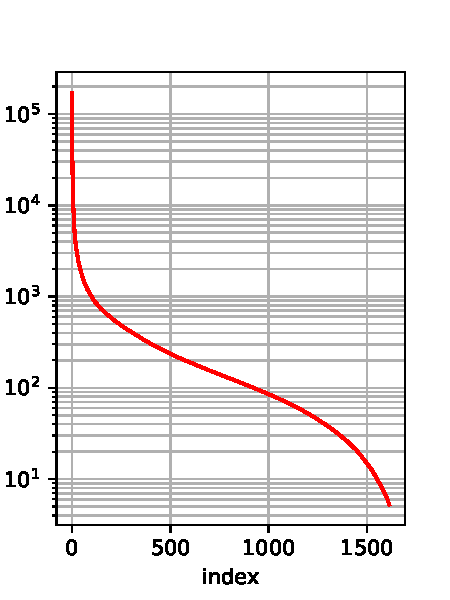
\includegraphics{image/singular_values.pdf}}

    \vspace*{-11em}\hfill
    \begin{tabular}{cccc}
      $r=1$ & $r=2$ & $r=3$ & $r=4$ \\
      \resizebox{0.15\textwidth}{!}{
\includegraphics{image/gray_picture_r1.pdf}} &
      \resizebox{0.15\textwidth}{!}{
\includegraphics{image/gray_picture_r2.pdf}} &
      \resizebox{0.15\textwidth}{!}{
\includegraphics{image/gray_picture_r3.pdf}} &
      \resizebox{0.15\textwidth}{!}{
\includegraphics{image/gray_picture_r4.pdf}} \\
    \end{tabular}
  \end{itemize}
\end{frame}

\begin{frame}[t,fragile]{特異値分解による画像圧縮}
  \begin{itemize}
  \item 特異値の分布とランク$r$近似 ($1614 \times 2178$グレイスケール写真)
    
    \hspace*{-3em}\resizebox{0.27\textwidth}{!}{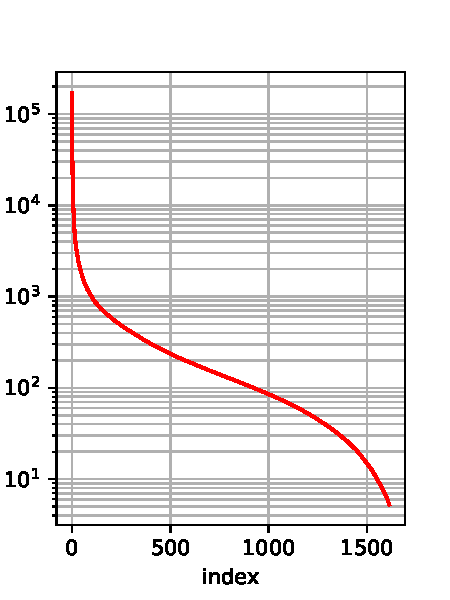
\includegraphics{image/singular_values.pdf}}

    \vspace*{-11em}\hfill
    \begin{tabular}{cccc}
      $r=1$ & $r=2$ & $r=3$ & $r=4$ \\
      \resizebox{0.15\textwidth}{!}{
\includegraphics{image/gray_picture_r1.pdf}} &
      \resizebox{0.15\textwidth}{!}{
\includegraphics{image/gray_picture_r2.pdf}} &
      \resizebox{0.15\textwidth}{!}{
\includegraphics{image/gray_picture_r3.pdf}} &
      \resizebox{0.15\textwidth}{!}{
\includegraphics{image/gray_picture_r4.pdf}} \\
      $r=5$ & $r=10$ & $r=20$ & $r=50$ \\
      \resizebox{0.15\textwidth}{!}{
\includegraphics{image/gray_picture_r5.pdf}} &
      \resizebox{0.15\textwidth}{!}{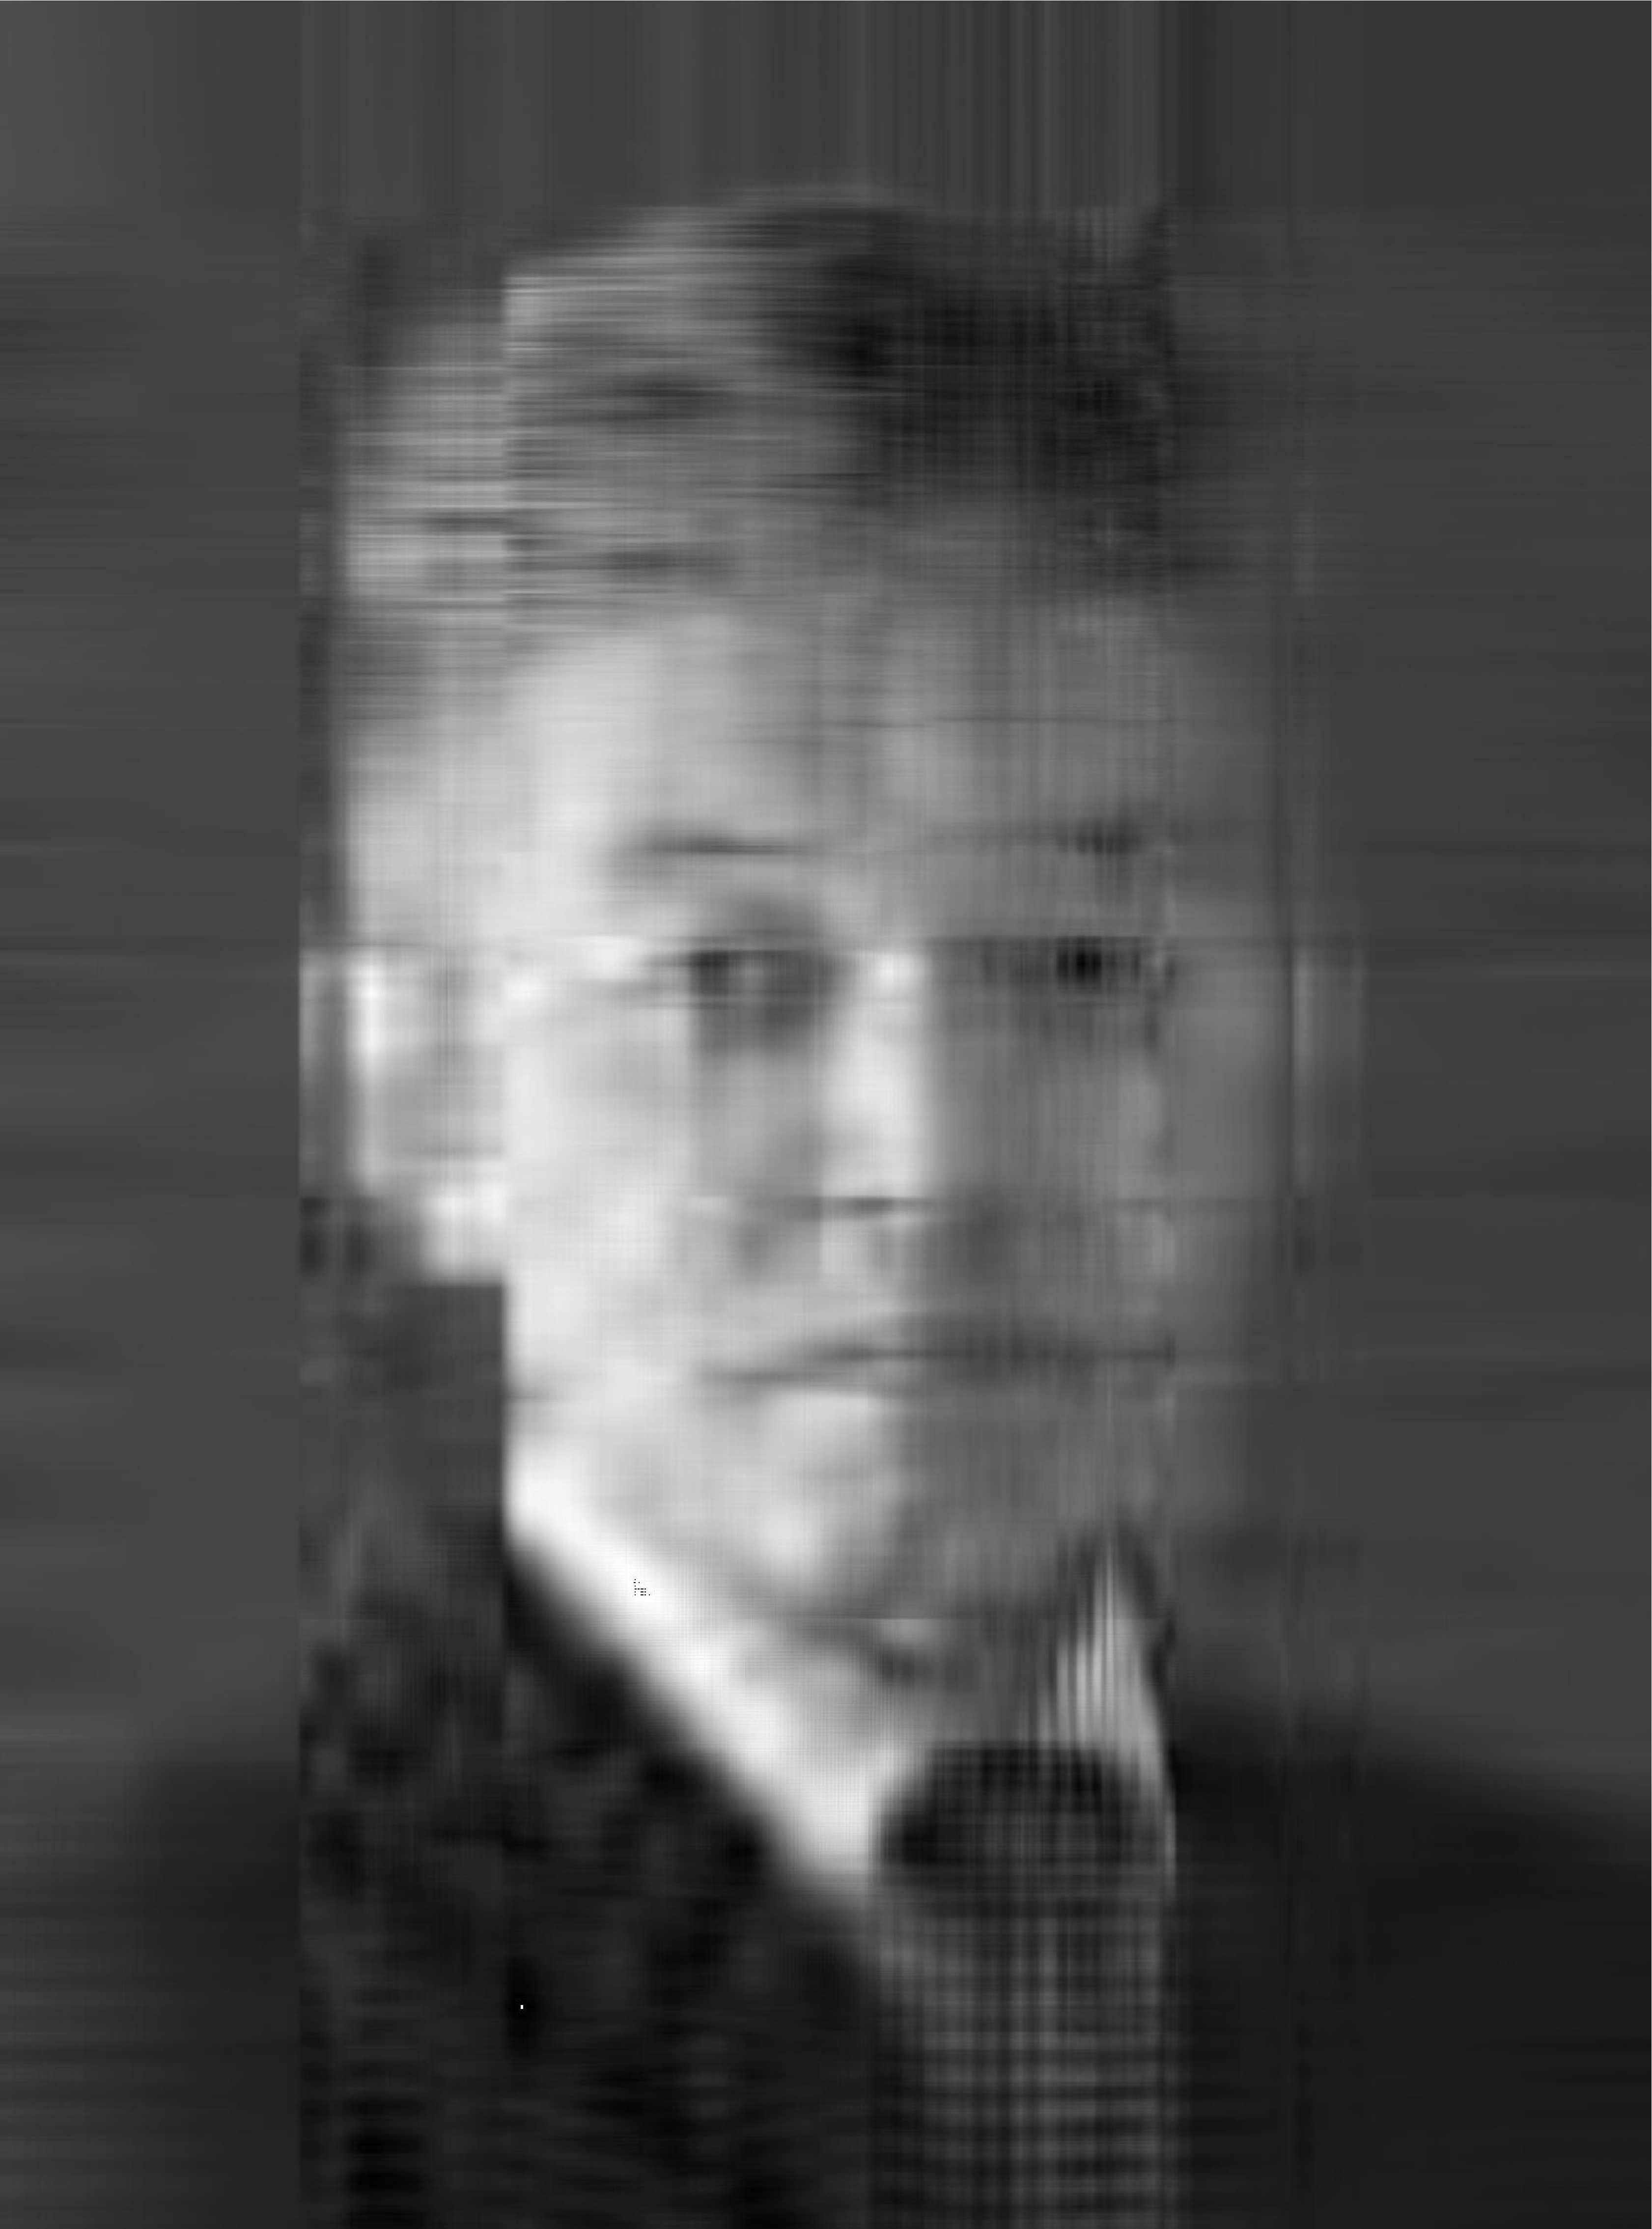
\includegraphics{image/gray_picture_r10.pdf}} &
      \resizebox{0.15\textwidth}{!}{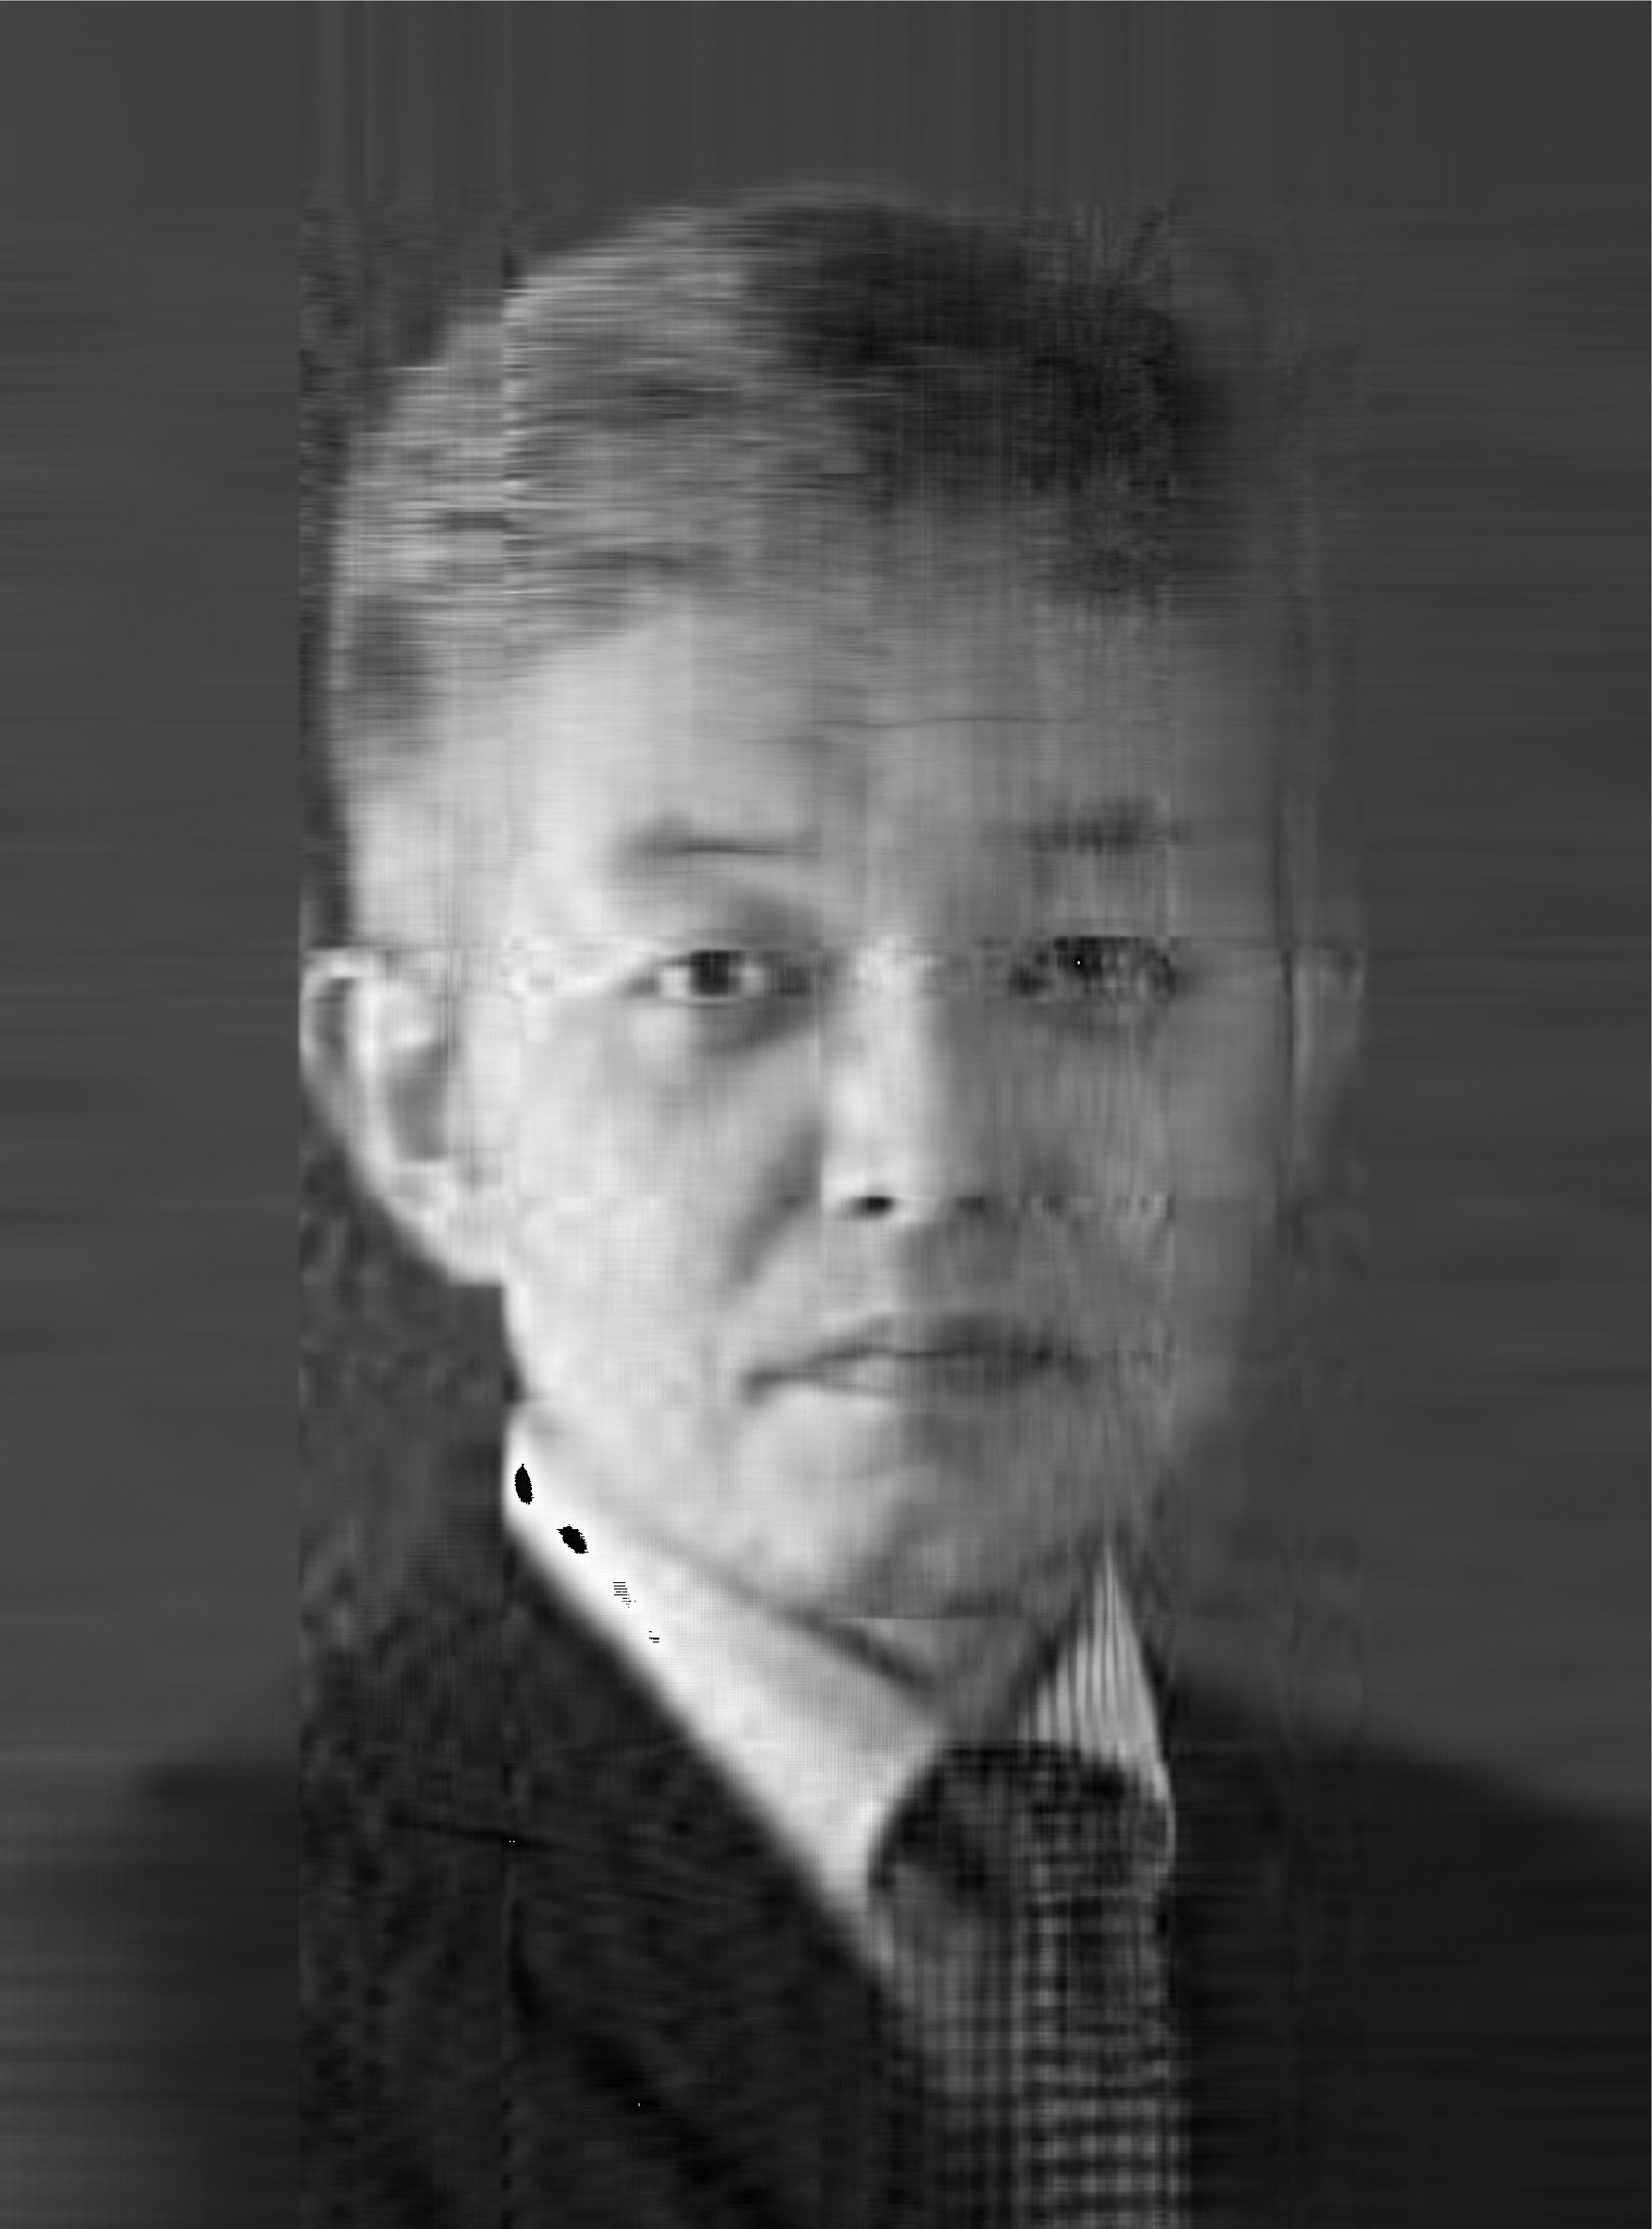
\includegraphics{image/gray_picture_r20.pdf}} &
      \resizebox{0.15\textwidth}{!}{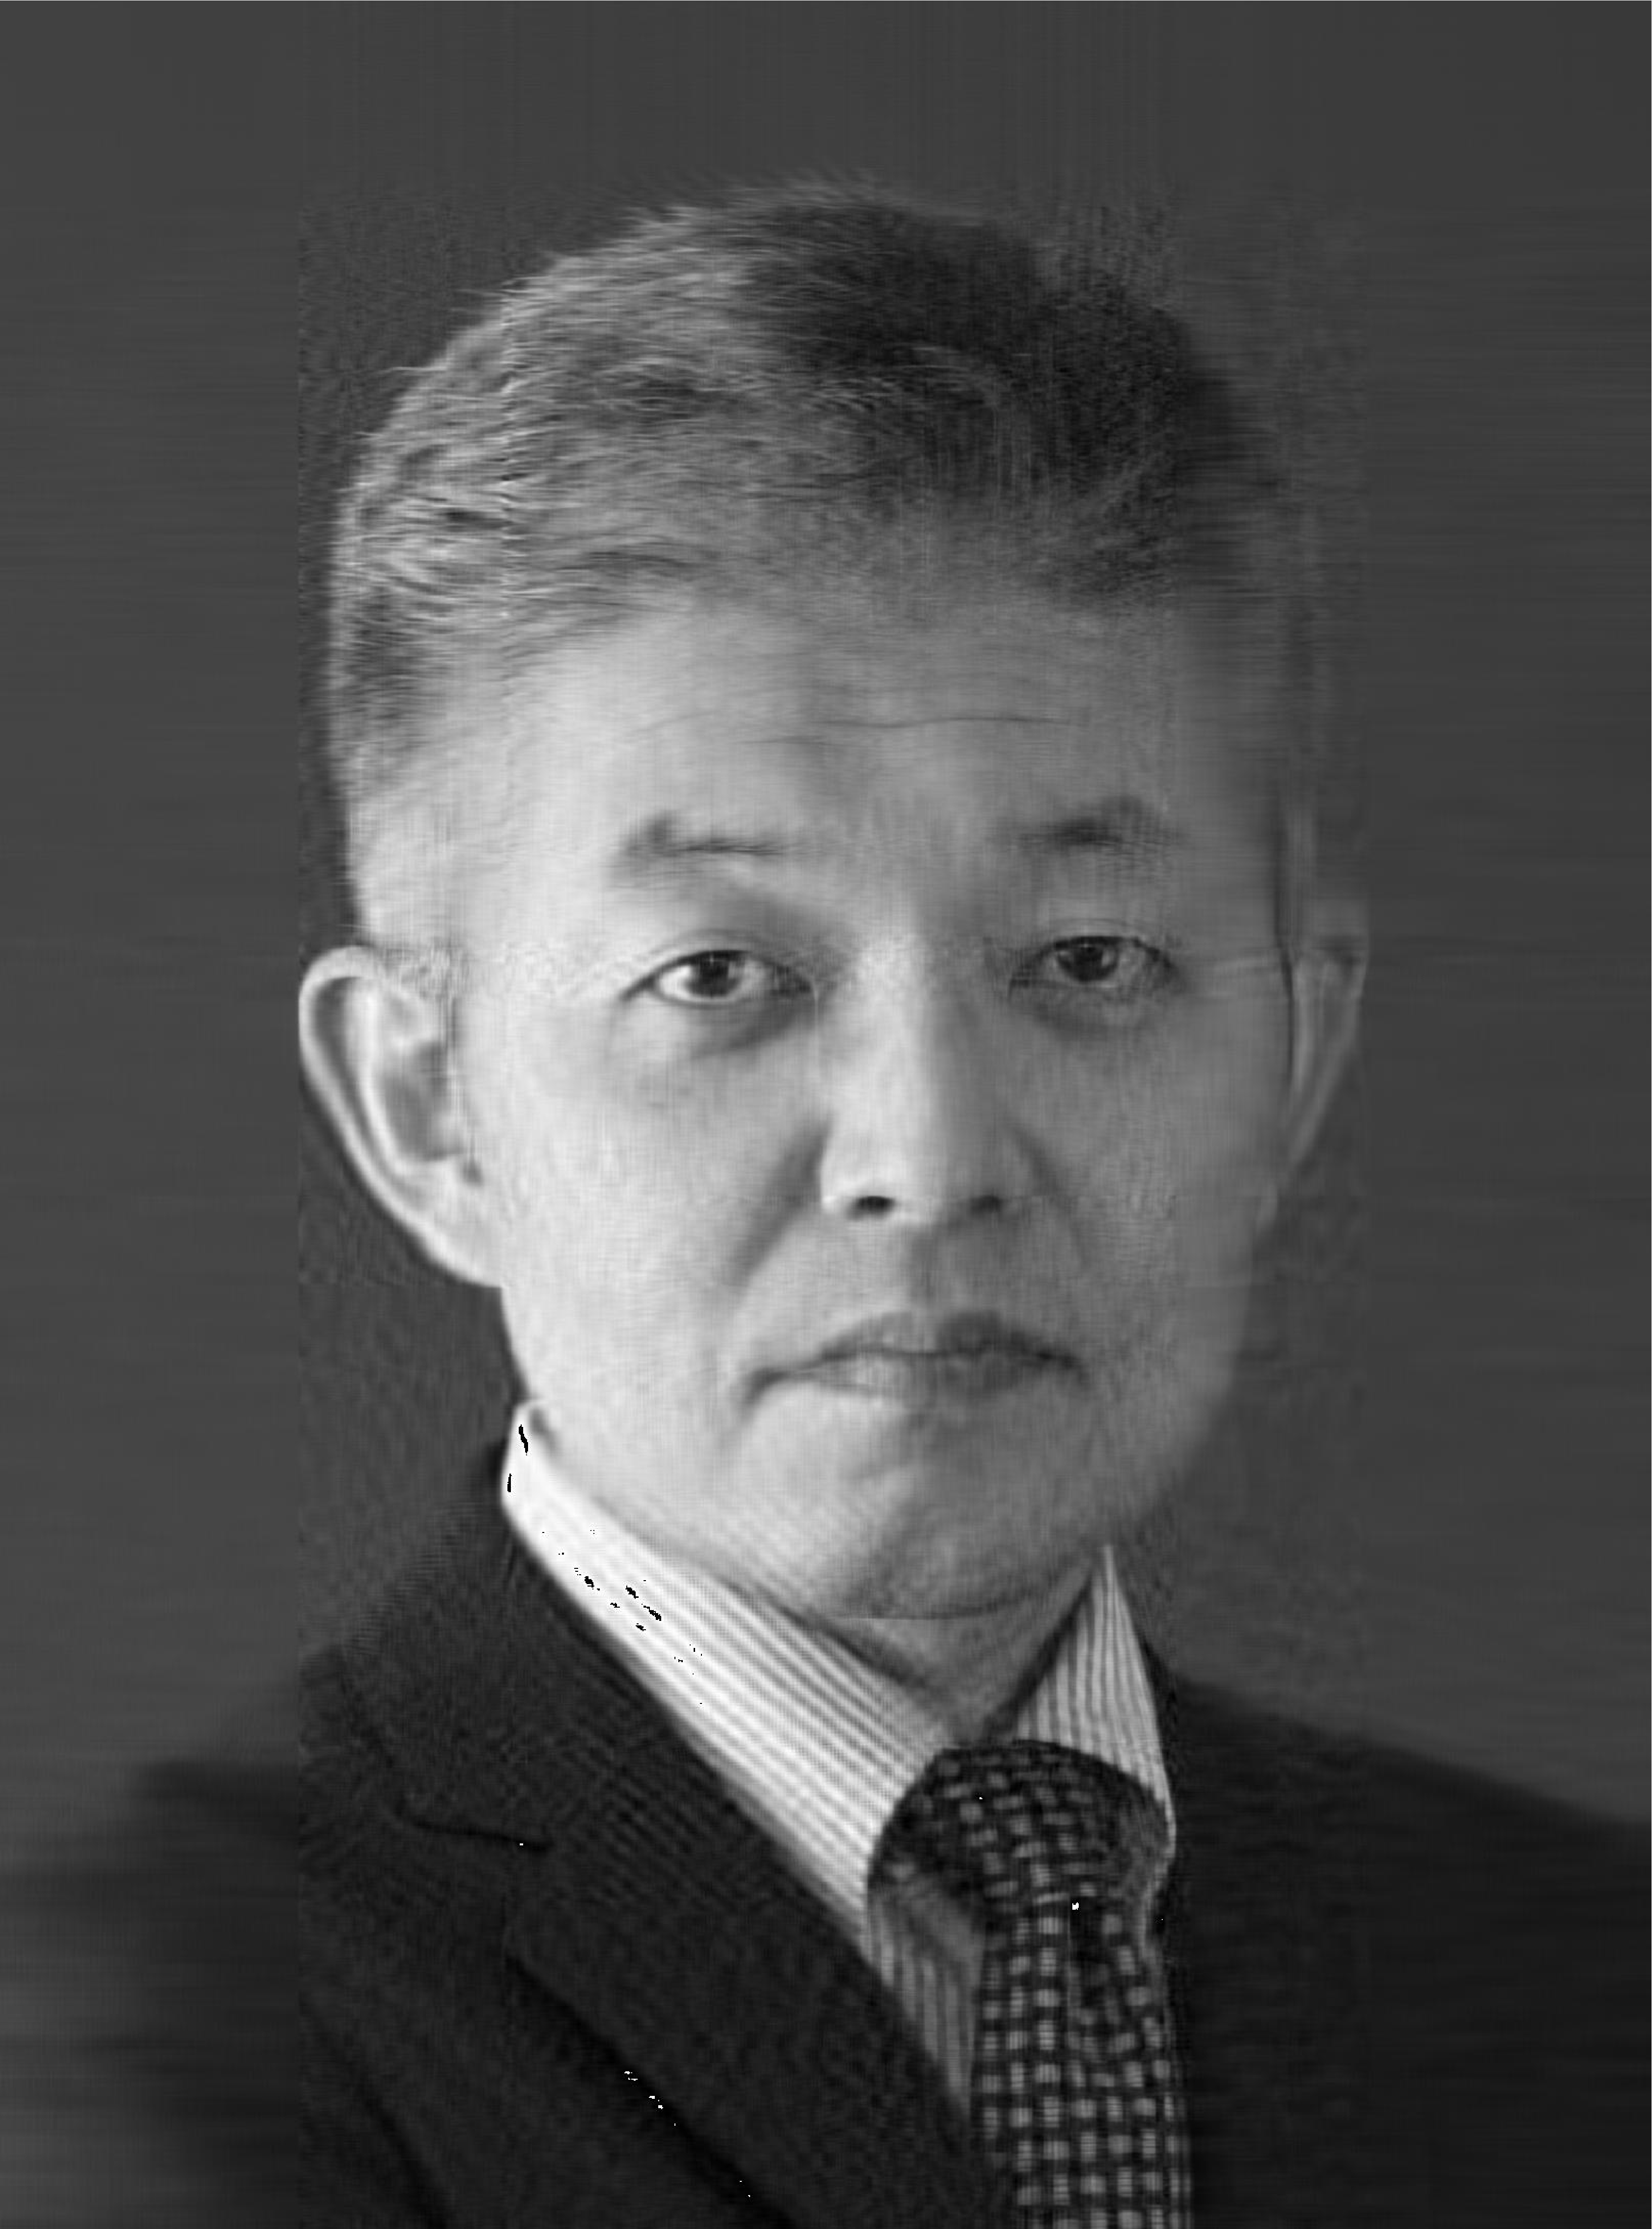
\includegraphics{image/gray_picture_r50.pdf}} \\
    \end{tabular}
  \end{itemize}
\end{frame}


\section{最小二乗法による回帰分析}

\begin{frame}[t,fragile]{最小二乗法によるフィッティング}
  \begin{itemize}
    %\setlength{\itemsep}{1em}
  \item 説明変数(例: 電圧): $x_1,x_2,x_3,\cdots,x_n$
  \item 観測値(例: 電流): $y_1,y_2,y_3,\cdots,y_n$
  \item 単回帰モデル: $y=a+bx+\epsilon$ \ \ ($\epsilon$: ノイズ)
  \item 未知母数: $a,b$
  \item 最小二乗法:
    残差$\displaystyle R(a,b) = \sum_i^n (y_i - (a+bx_i))^2$を最小化
    \[
    \begin{split}
      \frac{\partial R}{\partial a} &= - 2 \sum_i^n (y_i - (a+bx_i)) = 0 \\
      \frac{\partial R}{\partial b} &= - 2 \sum_i^n (y_i - (a+bx_i))x_i = 0
    \end{split}
    \]
  \end{itemize}
\end{frame}

\begin{frame}[t,fragile]{回帰分析の一般化}
  \begin{itemize}
    %\setlength{\itemsep}{1em}
  \item 基底関数: $\phi_j(x)$ \ \ ($j=1 \cdots m$)
  \item モデル: $\displaystyle y(x) = \sum_j^m \phi_j(x) w_j + \epsilon$
  \item 残差: $\displaystyle R({\bf w}) = \sum_i^n \Big[y_i - \sum_j^m \phi_j(x_i) w_j\Big]^2$
    \[
    \frac{\partial R}{\partial w_k} = -2 \sum_i^n \Big[ y_i - \sum_j^m \phi_j(x_i) w_j\Big] \phi_k(x_i) = 0 \qquad (k = 1\cdots m)
    \]
  \item 計画行列(design matrix) $\Phi_{ij} = \phi_j(x_i)$を導入すると
    \[
    R({\bf w}) = | {\bf y} - \Phi {\bf w} |^2
    \]
  \item 最小二乗解: $\Phi^{\rm t} \Phi {\bf w} = \Phi^{\rm t} {\bf y} \ \ \Rightarrow \ \
{\bf w} = (\Phi^{\rm t} \Phi)^{-1}\Phi^{\rm t} {\bf y}$
  \end{itemize}
\end{frame}

\begin{frame}[t,fragile]{リッジ回帰(Ridge Regression)}
  \begin{itemize}
    %\setlength{\itemsep}{1em}
  \item 基底関数の数(例: 多項式の次数)を増やしすぎると過学習 (over-fitting)」が生じる
  \item 正則化最小二乗法 ($\lambda$は非負の定数)
    \begin{align*}
    R({\bf w}) &= \sum_i^n \Big[y_i - \sum_j^m \phi_j(x_i) w_j\Big]^2 + {\color{red} \lambda} \sum_j^m w_j^2 \\
    &= | {\bf y} - \Phi {\bf w} |^2 + \lambda {\bf w}^{\rm t} {\bf w}
    \end{align*}
  \item 最小二乗解
    \[
    (\Phi^{\rm t} \Phi + \lambda \, {\rm I}) {\bf w} = \Phi^{\rm t} {\bf y} \ \ \Rightarrow \ \ 
      {\bf w} = (\Phi^{\rm t} \Phi + \lambda \, {\rm I})^{-1}\Phi^{\rm t} {\bf y}
      \]
  \end{itemize}
\end{frame}


\begin{frame}[t]{講義日程(予定)}
  \begin{itemize}
    % \setlength{\itemsep}{1em}
  \item 全8回 (水曜2限 10:25-11:55)
    \begin{itemize}
    \item 4月6日 講義1: 講義の概要・基本的なアルゴリズム
    \item 4月13日 演習1: 環境整備・C言語プログラミング・図のプロット
    \item 4月20日 講義2: 常微分方程式
    \item 4月27日 演習2 (グループ1): 基本的なアルゴリズム・常微分方程式
    \item 5月11日 演習2 (グループ2): 基本的なアルゴリズム・常微分方程式
    \item {\color{gray} 5月18日 休講}
    \item 5月25日 講義3: 連立方程式
    \item 6月1日 演習3 (グループ1): 連立方程式
    \item 6月8日 演習3 (グループ2): 連立方程式
    \item {\color{gray} 6月15日 休講}
    \item {\color{gray} 6月22日 休講}
    \item 6月29日 講義4: 行列の対角化
    \item 7月6日 演習4 (グループ1): 行列の対角化
    \item 7月13日 演習4 (グループ2): 行列の対角化
    \end{itemize}
  \item 2回目以降の演習はクラスを2グループに分けて実施(グループ1: 学生証番号が奇
数、グループ2: 偶数)
  \end{itemize}
\end{frame}

\end{document}
